\chapter{Implementation and Experiments}

In this chapter, we will show how the system specified in the Chapter 4 was implemented and what were the technologies used. We will also describe the experiments made and analyse the results obtained in comparison to existing solutions. Finally, we will discuss the difficulties found in the implementation and experimentation process.

\section{Used Technologies}
The Graph Aggregator (GA) algorithm was implemented using Python programming language, in version 2.7. The original data and the aggregate graphs were stored in a Neo4J database. In order to connect the GA to the Neo4J database, it was necessary to use the Python library Py2Neo, in version 3.1.2. The Analytical Query Processor uses the compiler built in Neo4J and the query accepted as input to the system is written using Cypher query language.

As mentioned in Chapter 2, Neo4J is the most popular graph database in the industry according to DB Engines website. In comparison with other DBs from the same category, Neo4J has a good performance considering time to process a query and the amount of memory consumed by the database.

The queries submitted to Neo4J are written in Cypher \cite{Neo4jCypher}, which is a declarative query language inspired by SQL and that describes graph patterns using ASCII characters. Figure \ref{fig:figure29} shows an example of how Cypher represents a relationship in the query syntax. This language also allows to create, update and delete vertices and edges. Since Cypher uses the terms ``nodes" and ``relationships" to refer to ``vertices'' and ``edges'' respectively, we will interchange these words accordingly throughout the text from now on.

\begin{figure}[ht]
\centering
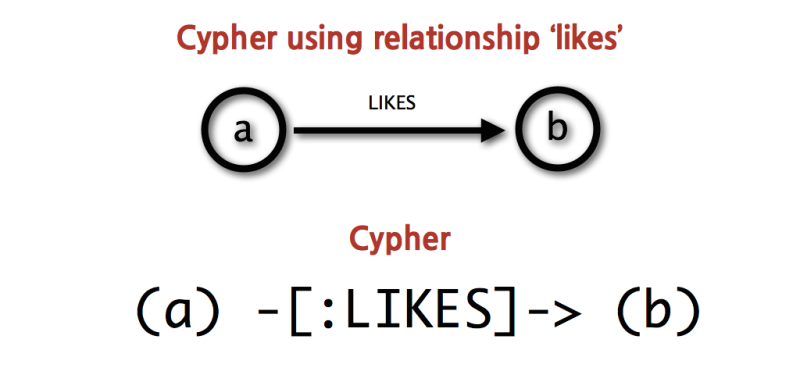
\includegraphics[width=0.6\textwidth]{../cypher_pattern_simple.png}
\caption{Cypher syntax representation of a relationship in the graph \cite{Neo4jCypher}}
\label{fig:figure29}
\end{figure}

Neo4J query language also includes a series of clauses and expressions similar to SQL, such as  $WHERE$, $ORDER BY$, $LIMIT$, $AND$, among others. The Cypher query shown in Figure \ref{fig:figure30} is an example of the general syntax of the language and it shows how it is possible to restrict the results by a certain threshold using the clause $WHERE$. The mentioned query will return a subgraph containing the nodes with labels $Label1$ and $Label2$ that have a relationship of type $TYPE$ with a property value above a certain threshold.

\begin{figure}[ht]
\centering
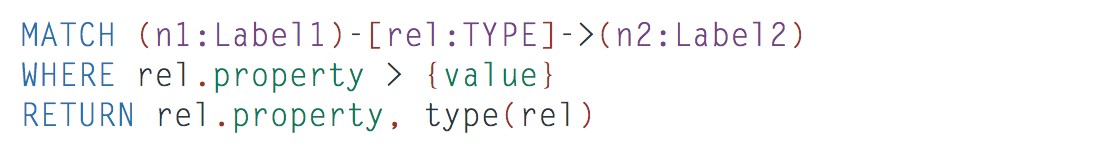
\includegraphics[width=0.8\textwidth]{../cypher_general_syntax.png}
\caption{Example of Cypher Query syntax \cite{Neo4jCypher}}
\label{fig:figure30}
\end{figure}

The data stored in a Neo4J database can be accessed using a Java API or a REST API by default. In order to facilitate the access to the data using a Python application we used an external library called Py2Neo, which wraps REST API requests to execute Cypher commands on the database. In this way, it was possible to implement the algorithm for the Graph Aggregators, where it consumes the original data, generate an aggregate graph and stores it in another instance of a Neo4J database.

Another interesting feature in Neo4J is its web-based user interface. This interface provides a direct way to submit Cypher queries to the database and a visualisation of the results. Figure \ref{fig:figure31} is a screenshot of the interface, showing the result of a simple query submitted in the text area at the top of the screen. The submitted query returns a subgraph showing the relationship between the Author Felix Naumann with all his publications present in the database. The interface shows each node as a circle and relationship as an arrow, it also shows the properties and labels of nodes and relationships when they are clicked. The experiments shown in this chapter will be displayed using the graphic interface provided by Neo4J.

\begin{figure}[ht]
\centering
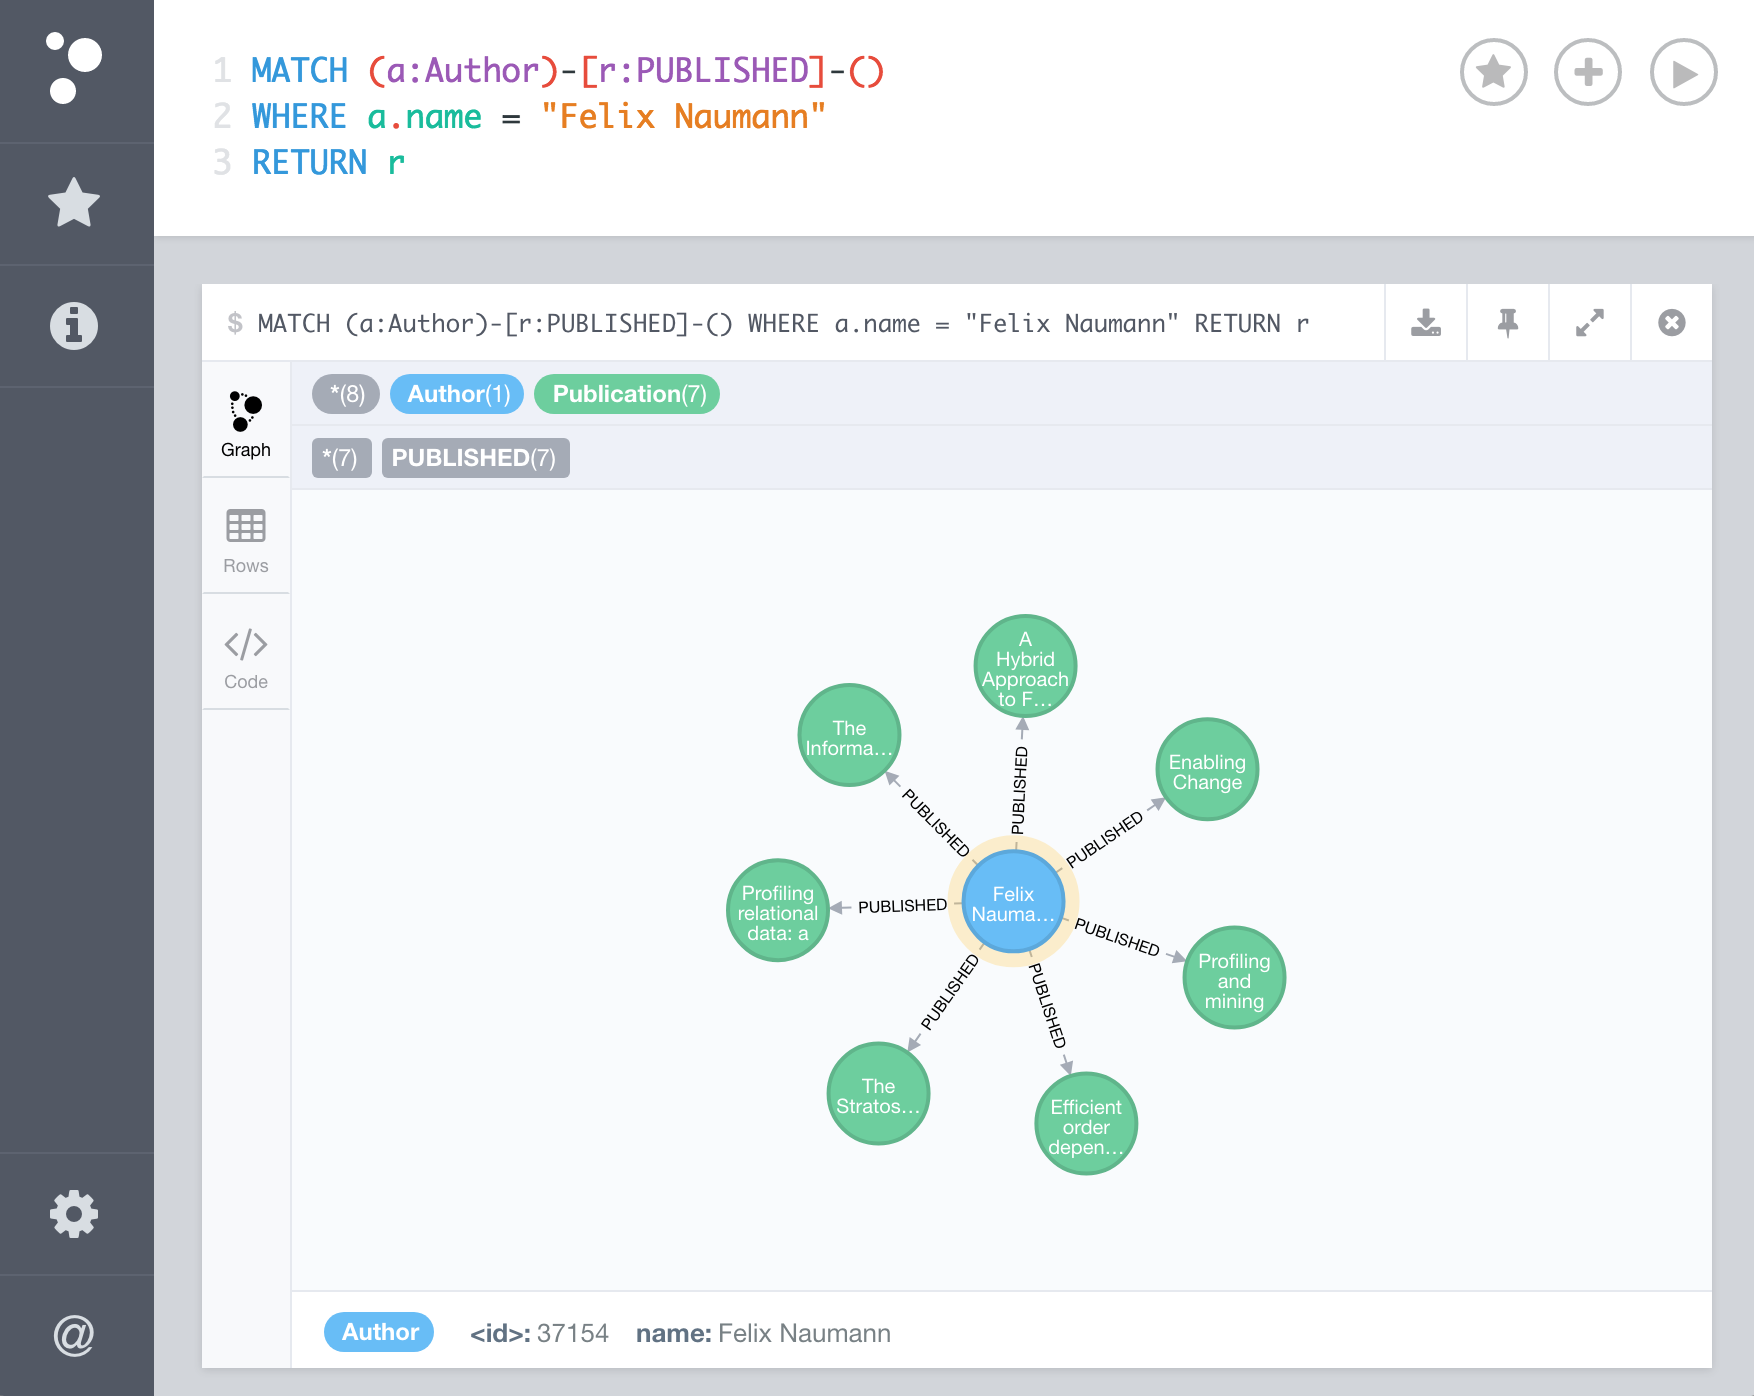
\includegraphics[width=1\textwidth]{../neo4j_user_interface.png}
\caption{Neo4J User Interface}
\label{fig:figure31}
\end{figure}

\section{Dataset}

The dataset used for the experiments was the Database System and Logic Programming (DBLP) computer science bibliography, available in (http://dblp.uni-trier.de/db/), which contains more than 3.8 million publications published by more than 1.7 million authors. The dataset can be downloaded as a XML file accompanied by a DTD file that describes the schema of the data. The Listing in \ref{lst:listing1} is an excerpt of the DBLP XML file showing how a publication is structured in the document.

\lstset{breaklines=true,
	caption={DBLP XML File Excerpt},
	label={lst:listing1},
	captionpos=b, 
	frame=single,
	morekeywords={article, author, title, pages, year, volume, journal, number, ee, url, mdate, key}}

\begin{lstlisting}
<article mdate="2017-01-03" key="journals/jacm/GanorKR16">
  <author>Anat Ganor</author>
  <author>Gillat Kol</author>
  <author>Ran Raz</author>
  <title>Exponential Separation of Information and Communication for Boolean Functions.</title>
  <pages>46:1-46:31</pages>
  <year>2016</year>
  <volume>63</volume>
  <journal>J. ACM</journal>
  <number>5</number>
  <ee>http://dl.acm.org/citation.cfm?id=2907939</ee>
  <url>db/journals/jacm/jacm63.html#GanorKR16</url>
</article>
\end{lstlisting}

The excerpt shown in Listing  \ref{lst:listing1} refers to an article published in J. ACM journal and it contains information about the article's authors, title, pages in journal, year of publication and other informations about the journal's volume, number and electronic edition location. Each publication also has a unique key and the date of the last modification as attributes and an element with the url of the publication in the DBLP website. Besides journal articles, the DBLP dataset also contains books, thesis, conferences and workshop papers, among others.

Once the XML file was downloaded, all the data was parsed and stored into a SQLite database. In order to have a more controlled environment for the experiments, we selected a subset of the original data, considering only papers and articles published in the following venues since 2014:

\begin{itemize}
\item SIGMOD International Conference on Management of Data (SIGMOD)
\item Brazilian Symposium on Databases (SBBD)
\item International Conference on Very Large Databases (VLDB)
\item IEEE International Conference on Data Engineering (ICDE)
\item World Wide Web: Internet and Web Information Systems (WWW)
\end{itemize}

The selected subset of publications was imported to a Neo4J instance, following the schema depicted in Figure \ref{fig:figure32}. Each publication became a node in the graph database, with three attributes: (i) the title; (ii) the year of publication and (iii) the acronym of the venue. The authors of each publication also became a node, uniquely identified by the name of the author, and they are connected with the publications node by a relationship of type PUBLISHED. Authors that have contributed in the same publication are also connected by a relationship of type CO\_AUTHORSHIP.

\begin{figure}[ht]
\centering
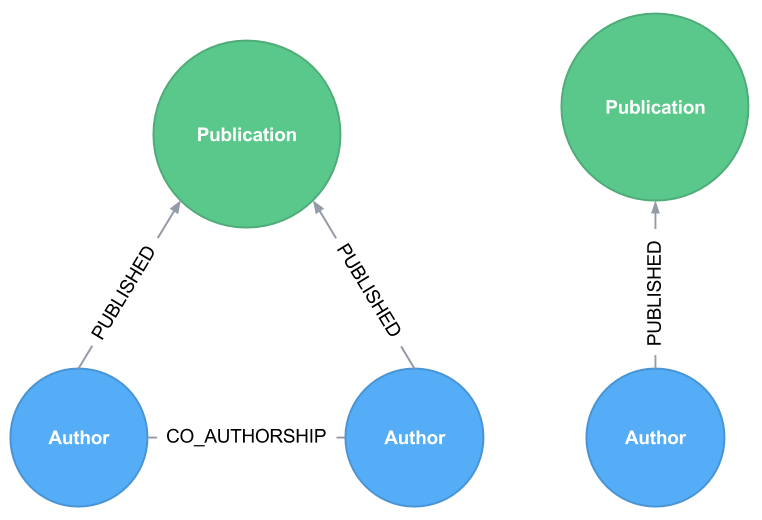
\includegraphics[width=0.6\textwidth]{../dblp_schema.png}
\caption{DBLP dataset schema in graph database}
\label{fig:figure32}
\end{figure}

By the end of the DBLP subset loading process to Neo4J, we had 887 Publication nodes, 2.398 Author nodes, 6.754 PUBLISHED relationships and 25.572 CO\_AUTHORSHIP relationships.

\section{Experiments and Results}

With the Neo4J database loaded with DBLP data, we executed the Graph Aggregator (GA) algorithm passing as parameters the dimensions year and venue of a Publication node and the COUNT aggregate function. Figure \ref{fig:figure33} shows a subgraph of the aggregate graph generated by the GA, with one aggregate node representing all the publications on ICDE 2016 and some of the authors that published on that conference, that year. From the measure attribute of the aggregate node, we know that ICDE had 60 publications in 2016.

\begin{figure}[!h]
\centering
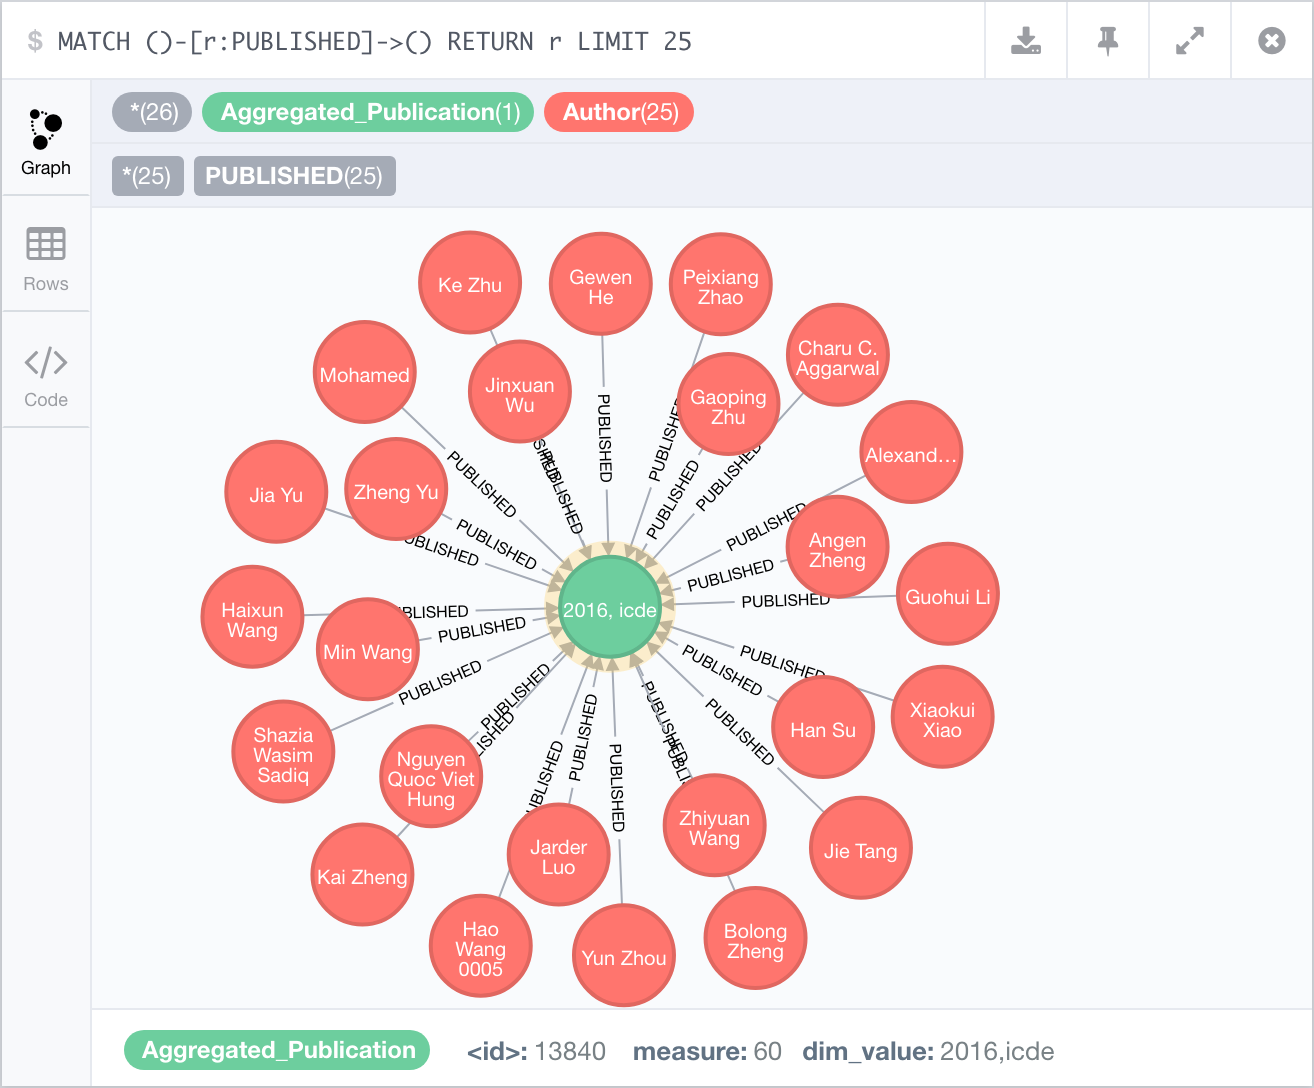
\includegraphics[width=0.8\textwidth]{../aggregate_graph_subgraph.png}
\caption{Subgraph from the Aggregate Graph generated by the GA}
\label{fig:figure33}
\end{figure}

Once we generated the aggregate graph, we were able to do an experiment to evaluate the effectiveness of the proposed system. For that, we submitted queries to calculate the three types of supported measures: content-based, graph-specific and graph as measure.

\subsection{Content-based Measure}

For this type of measure, we submitted a query asking for the amount of publications by venue in the year of 2016. This query was submitted to the aggregate graph generated by the GA and it returns all the nodes with the label Aggregate\_Publication where the dimension year has the value 2016. The result is then ordered by the number of publications measure.

Figure \ref{fig:figure34} depicts the result of the query, listing the venues ordered by the amount of publications in the year of 2016. The conference SIGMOD appears at the top of the list with 61 publications for that year. In comparison to a traditional relational OLAP system, this query is corresponding to a slice operation, in which we slice a part of the venue dimension based on the value of the dimension year.

\begin{figure}[!h]
\centering
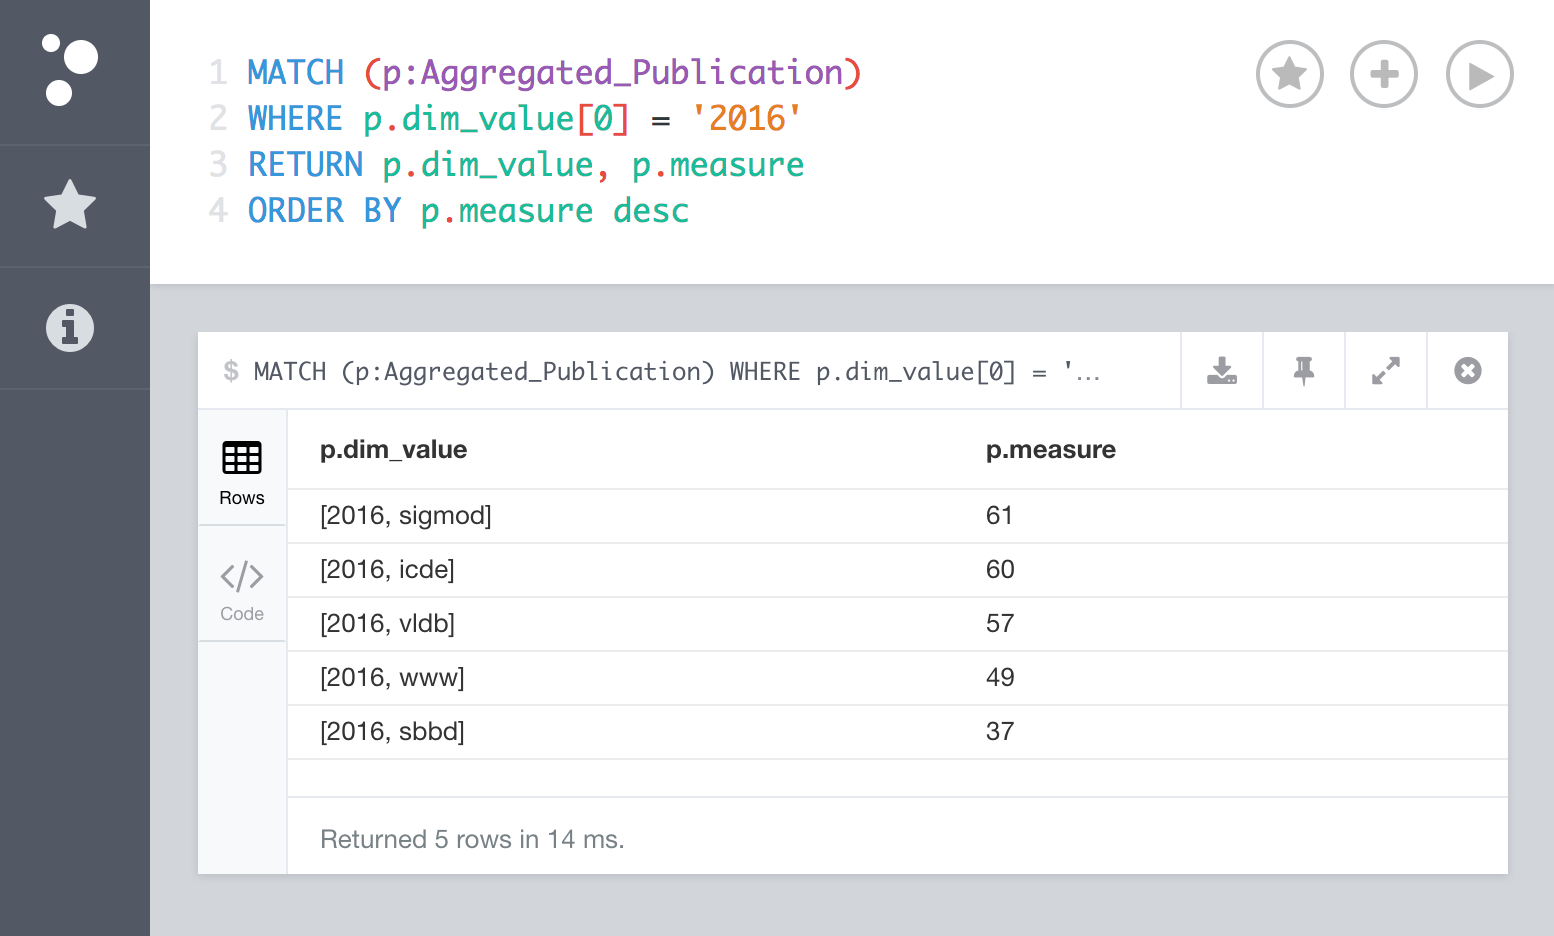
\includegraphics[width=0.8\textwidth]{../exp_content_measure.png}
\caption{Result of experiment with a content-based measure query}
\label{fig:figure34}
\end{figure}

\subsection{Graph-specific Measure}

In order to test this type of measure, we submitted two centrality measures queries to the original dataset in the graph database. The first measure calculated was the degree centrality of each Author node considering the CO\_AUTHORSHIP relationship. As mentioned in Chapter 2, the degree centrality is given by the number of adjacent node, i.e. the number of CO\_AUTHORSHIP relationship an Author node has.

Figure \ref{fig:figure35} shows the result of the centrality measure query, listing the 10 authors with the highest degree centrality in the original network. For our dataset, Michael J. Franklin is the author with the highest number of adjacent Author nodes, which means that he is one of the focal points in the network.

\begin{figure}[!h]
\centering
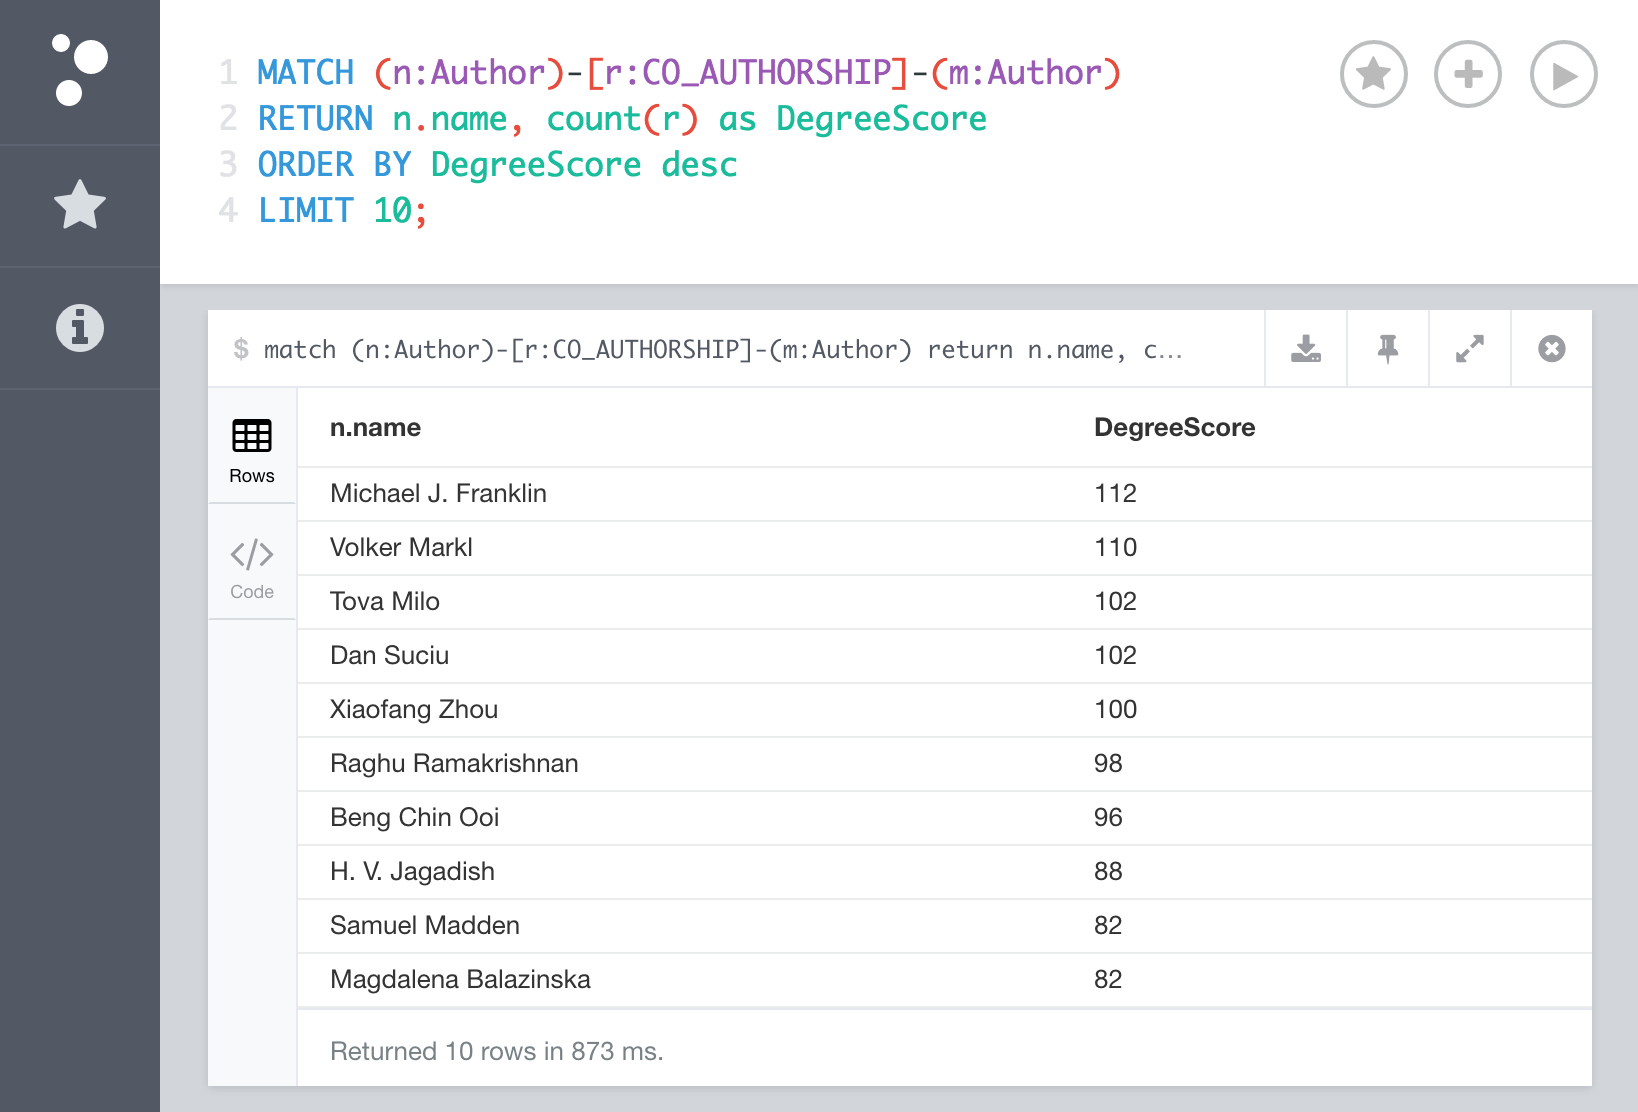
\includegraphics[width=0.8\textwidth]{../exp_degree_centrality.png}
\caption{Result of experiment with the degree centrality measure for Authors}
\label{fig:figure35}
\end{figure}

The second measure calculated was the betweenness centrality of the authors. This centrality measure is given by the frequency in which an author node appears in the shortest path of any other two author nodes in the graph. In Cypher, there is a built-in function to retrieve all shortest path between two nodes called $allShortestPaths$. Since getting all the shortest path between the combination of any 2 nodes in the graph is such a complex computation, we considered the paths with maximum 3 degrees of separation and we avoided inverse relationships by comparing the id of the nodes. Finally, we returned the 10 authors that most appeared in the list of the shortest paths.

Figure \ref{fig:figure36} shows the result of author's betweenness centrality calculation. Reaffirming his importance in the co-authorship network, Michael J. Franklin appears again in the first position of the list, meaning that he is an important point of collaboration between authors. One interesting result is related to the second place for both experiments: the second author with the highest degree centrality is not the same as the second author with the highest betweenness centrality. This means that, even so Volker Marki co-authored publications with more authors than Beng Chin Ooi, the latter is part of more collaboration chains between two other authors in the network.

\begin{figure}[!h]
\centering
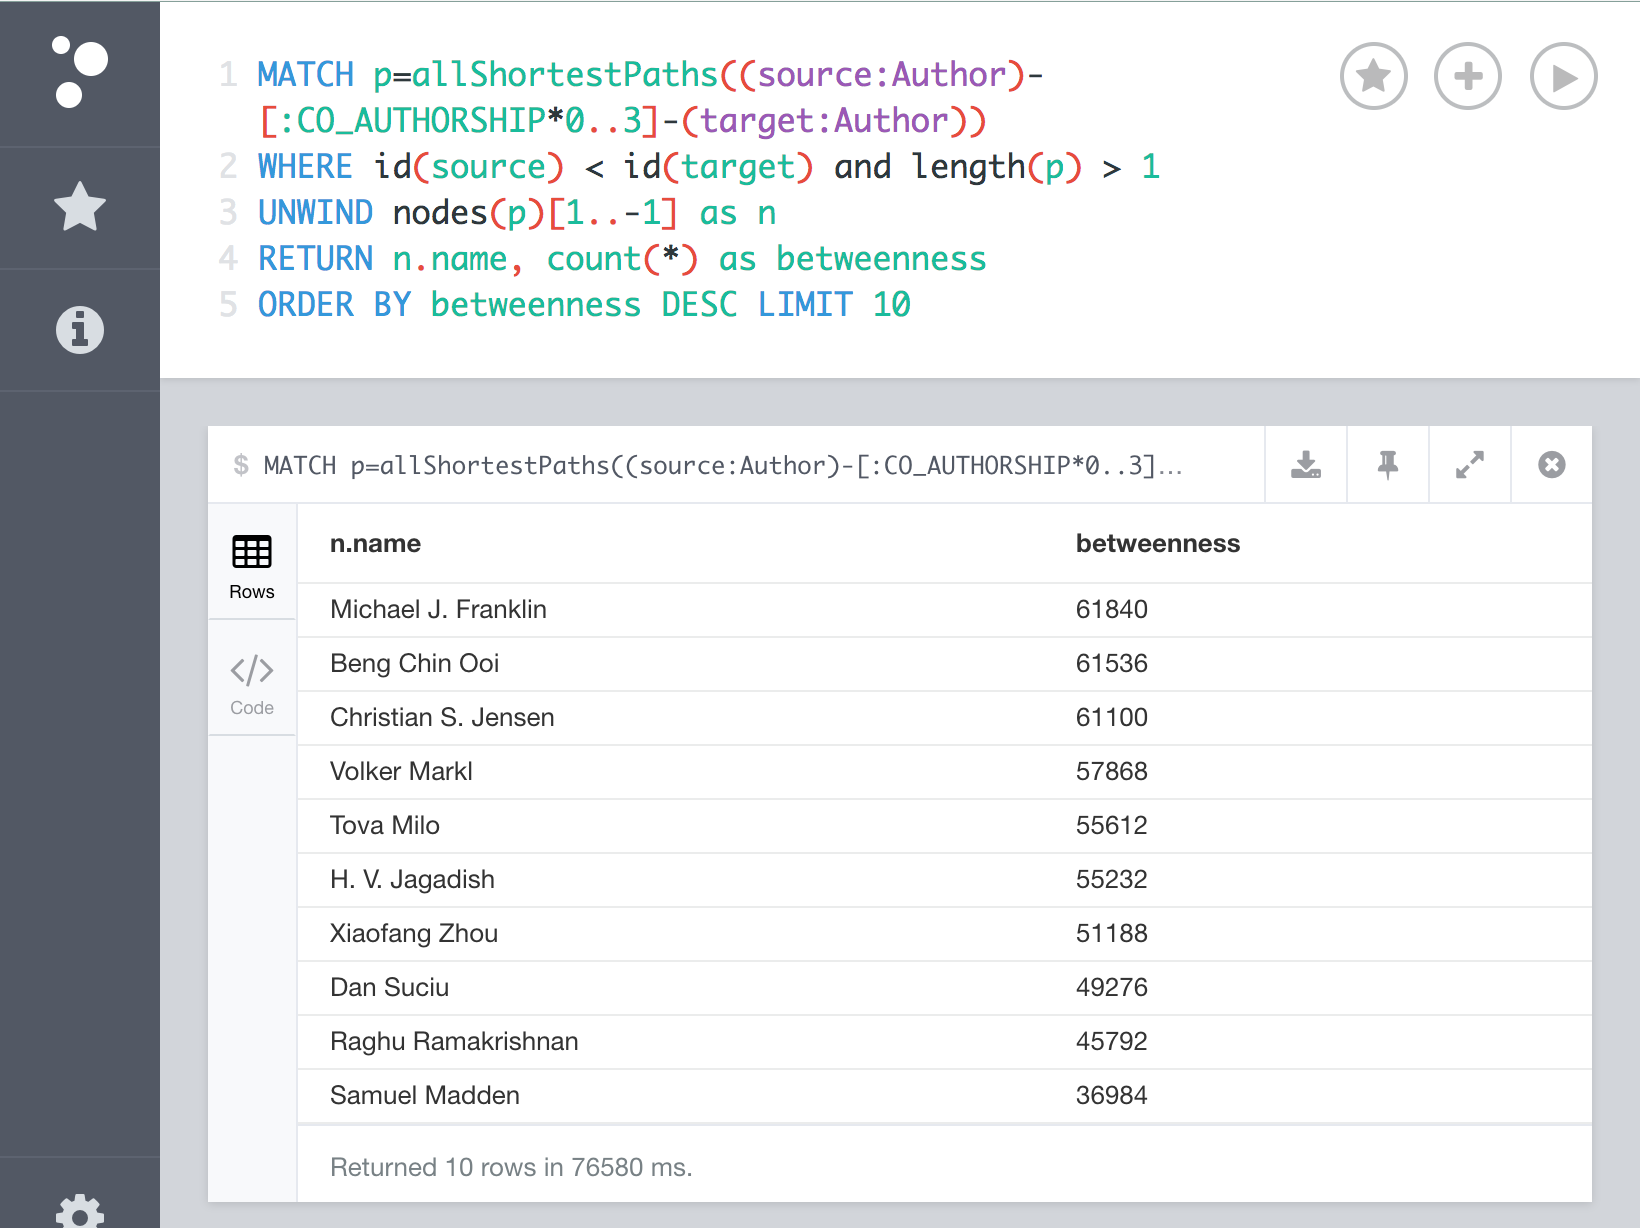
\includegraphics[width=0.8\textwidth]{../exp_betweenness_centrality.png}
\caption{Result of experiment with the betweenness centrality measure for Authors}
\label{fig:figure36}
\end{figure}

\subsection{Graph as Measure}
This type of measure is given by the aggregate graph itself, since it is a representation of data aggregated by dimensions. For our running example, this measure represents the topological disposition of the relationship between publications and authors when the data is aggregated according to the dimensions year and venue.  

Figure \ref{fig:figure37} shows a screenshot of a subgraph retrieved from the aggregate graph. The subgraph was limited to 400 relationships in order to facilitate the visualisation. From the screenshot we can notice the topology distribution of author nodes that published works on ICDE in 2016 and 2015, specially the authors that published in both editions of the conference.

\begin{figure}[!h]
\centering
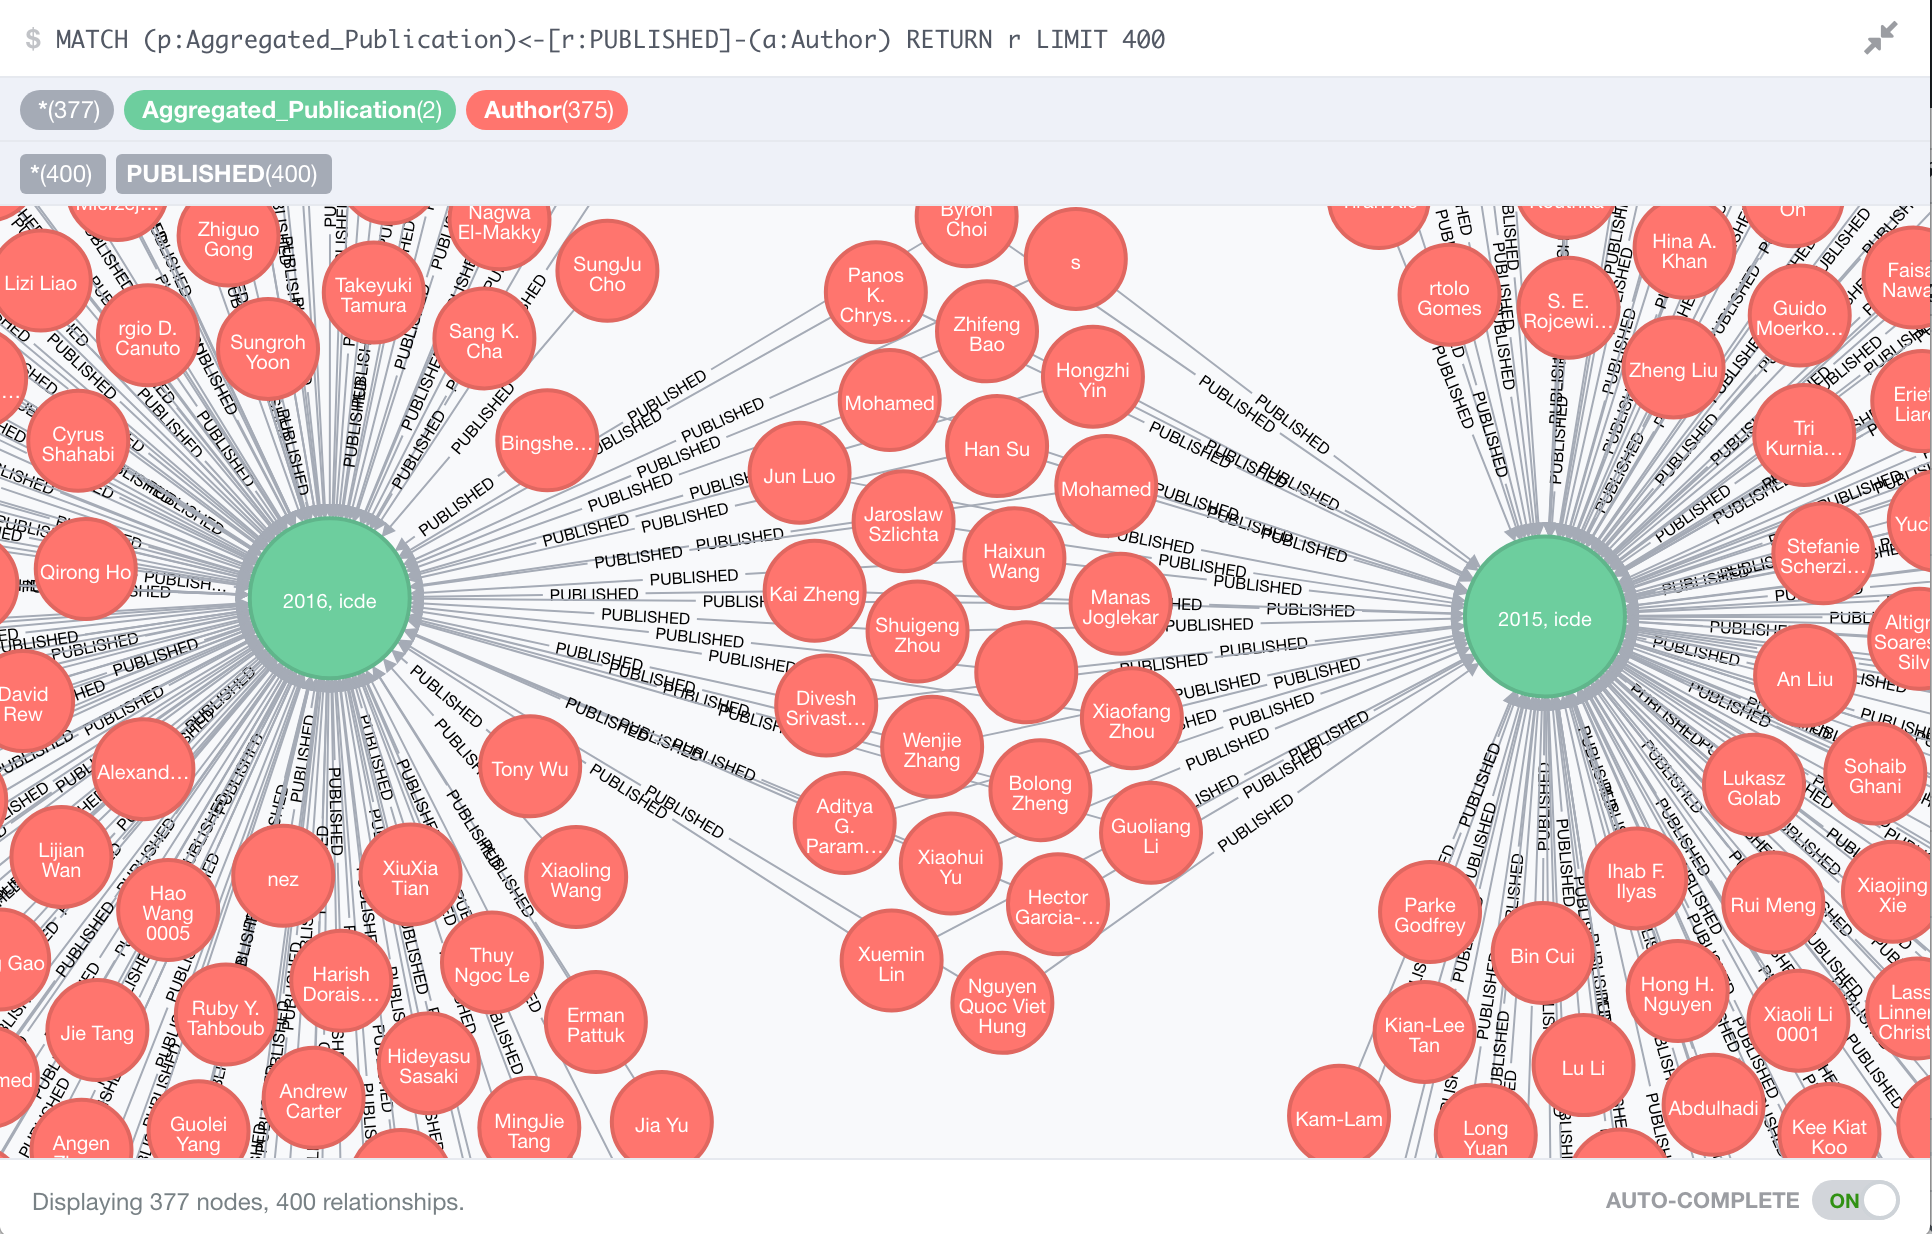
\includegraphics[width=1\textwidth]{../graph_measure.png}
\caption{Result of experiment with the graph as a measure}
\label{fig:figure37}
\end{figure}

\section{Result Analysis}
Given the results obtained from the experiments described in the previous section, we are able to confirm the effectiveness of the proposed system in supporting multidimensional analysis on graph database. The presented solution also supports the execution of graph-based analysis, such as centrality measures. In this way we are able to extract three different types of measures from the same origin data aggregated according to user defined dimensions.

In comparison to other works in this area, the proposed system gives full support for heterogeneous graphs without the need to change the original data schema. Focusing the comparison with the framework presented in \cite{Ghrab2013}, our system is able to answer the same types of query without the extra step to change the data model of our original dataset. Table \ref{tb:table2} summarises the comparison between existing frameworks and our proposed system.

\begin{table}[!ht]
\setlength\extrarowheight{2pt}
\caption{Comparison between existing frameworks and our proposed system}
\label{tb:table2}
\begin{tabularx}{\textwidth}{|Y|Z|Z|Z|}
\hline
\cellcolor[HTML]{C0C0C0}\textbf{Framework} & \cellcolor[HTML]{C0C0C0}\textbf{Graph} & \cellcolor[HTML]{C0C0C0}\textbf{Dimensions} & \cellcolor[HTML]{C0C0C0}\textbf{Operations}\\\hline
{\cellcolor[HTML]{EFEFEF} Graph Cube} & Homogeneous & Vertex Attributes & Cuboid and Crossboid Query\\\hline
{\cellcolor[HTML]{EFEFEF} Graph OLAP} & Homogeneous & Informational and Topological & I-OLAP and T-OLAP Operations\\\hline
{\cellcolor[HTML]{EFEFEF} HMGraph} & Heterogeneous & Informational, Topological and Entity & I-OLAP, T-OLAP, Rotate and Stretch Operations\\\hline
{\cellcolor[HTML]{EFEFEF} Pagrol} & Homogeneous & Vertex and Edge Attributes & 3 Query Category and Roll-up/Drill-down Operations \\ \hline
{\cellcolor[HTML]{EFEFEF} GRAD Graph Cubes} & Heterogeneous & Inter-class and Intra-class & - \\ \hline
{\cellcolor[HTML]{EFEFEF} \textbf{Using OLAP Queries for Data Analysis on Graph Databases}} & \textbf{Heterogeneous} & \textbf{Vertex and Edge Attributes} & \textbf{OLAP Operations and Network Analysis Algorithms} \\ \hline
\end{tabularx}
\end{table}

\section{Difficulties Found}

Unfortunately, we are unable to provide a more precise comparison between the framework in \cite{Ghrab2013} and our proposal due to the lack of experiment description. A similar issue also applies to other works presented in Chapter 3, i.e. the state of the art for Graph Cubes and OLAP analysis on graph databases.

The published papers in this area fail in providing enough description on how the proposed solution was implemented and where the dataset used in the experiments is available. Furthermore, when experiments are presented in the paper, they only compare different version of the same framework. Until now, it hasn't been proposed an experiment that can be replicated amongst different frameworks.

The absence of a benchmark for experiments in this area makes the evaluation of the proposed system difficult. In order to compare ourselves to others, we can only rely on qualitative measures, based on the features presented by existing frameworks.

Another difficulty found during the implementation of the system was the size of the graph supported by Neo4J. The DBLP has more than 3.8 million publications, but we limited our dataset according to some conferences and journals, as mentioned before. At first, we wanted to conduct the experiments using at least 5.000 publications, but we were not able to load all the nodes and relationships to Neo4J. Our script to load the data kept getting error related to the communication with Neo4J REST API and we couldn't figure out how to fix it. In order to be able to finish all the experiments on time, we had to reduce the number of publications loaded to the database.

\section{Final Considerations}
In this chapter, we detailed how the system proposed by this work was implemented, specifying what were the technologies used in the process. The dataset used in the experiments was presented as well as the results obtained. Finally, we presented a qualitative comparison with existing solutions and listed the main difficulties found during the system's implementation.